\documentclass[11pt,a4paper]{article}
\usepackage[margin=2.5cm]{geometry}
\usepackage{setspace}
\usepackage{hyperref}
\usepackage{amsmath}
\usepackage{float}
\usepackage{graphicx}
\usepackage{booktabs}
\usepackage{subcaption}
\setstretch{1.15}
\usepackage[utf8]{inputenc}

\title{Mode Connectivity in Neural Networks: \\ Evaluating Permutation Alignment Methods via Controlled Benchmarks}
\author{Maciek Łodziński}
\date{February 4th, 2026}

\begin{document}
\maketitle

\begin{abstract}
We present a controlled experimental framework for evaluating permutation-finding methods in the context of linear mode connectivity (LMC). By constructing pairs of neural networks that are LMC-connected by design, applying known random permutations, and testing whether existing alignment methods can recover connectivity, we establish ground-truth benchmarks for assessing method capability. Our results show that weight matching achieves near-perfect alignment when models are close in parameter space, but performance degrades as the distance between modes increases—providing insights into the limitations of current methods and the validity of the one-basin hypothesis.
\end{abstract}

\section{Introduction}

The Entezari et al. (2021) conjecture posits that most SGD solutions belong to the same basin of the loss landscape when permutation symmetry is taken into account. Formally, for two independently trained networks $w_0$ and $w_1$, there should exist a permutation $P$ such that the linear interpolation between $w_0$ and $P(w_1)$ exhibits no loss barrier.

Testing this hypothesis directly is challenging: when alignment methods fail on independently trained models, we cannot distinguish between two possibilities:
\begin{enumerate}
    \item[(A)] No valid permutation exists (the hypothesis is false)
    \item[(B)] A valid permutation exists but methods cannot find it (methods are insufficient)
\end{enumerate}

To address this, we design a controlled benchmark where we \textit{know} a valid permutation exists by construction, allowing us to isolate method capability from hypothesis validity.

\section{Background}

\subsection{Linear Mode Connectivity}

Two networks $w_0$ and $w_1$ are said to be linearly mode connected (LMC) if the loss barrier along their linear interpolation is negligible:
\begin{equation}
    \text{barrier}(w_0, w_1) = \max_{\alpha \in [0,1]} \mathcal{L}(\alpha w_0 + (1-\alpha) w_1) - \frac{1}{2}(\mathcal{L}(w_0) + \mathcal{L}(w_1)) \approx 0
\end{equation}

\subsection{Permutation Symmetry}

Neural networks exhibit permutation symmetry: neurons within a layer can be reordered (along with corresponding input/output weights) without changing the function computed. For a permutation $P^*$ applied to network $w_1$, the permuted network $w_1' = P^*(w_1)$ computes the same function as $w_1$, but linear interpolation with $w_0$ typically yields high barriers due to neuron misalignment.

\subsection{Variance Collapse and REPAIR}

Jordan et al. (2023) identified that even with correct permutation alignment, linear interpolation suffers from \textit{variance collapse}: the variance of activations in interpolated networks decreases, causing performance degradation. They proposed REPAIR (REnormalizing Permuted Activations for Interpolation Repair), which rescales preactivations to restore proper statistics. This is particularly relevant at $t=0.5$ where variance differs most from the endpoints.


\section{Experimental Design}

\subsection{Creating LMC-Connected Pairs}

A critical requirement is that the shifted mode $w_1$ must be reachable by SGD. We considered several methods:

\begin{enumerate}
    \item \textbf{Continue training with different batch ordering} — Train $w_0$ for additional epochs with a different random seed for batch shuffling. This is unambiguously SGD-reachable and produces natural variation.
    
    \item \textbf{Shared initialization with split training} — Train a model for $N$ epochs, then create two copies and continue training each with different batch orderings - approach, used by Entezari et al. (2021).
    
    \item \textbf{Points along a Bézier curve} — While these points have low loss, they are optimized for path smoothness rather than being natural SGD solutions
    
    \item \textbf{Small perturbation + fine-tuning} — Adding noise and fine-tuning briefly. This often returns to near the original point, providing insufficient divergence.
    
    \item \textbf{Cyclic learning rate} — Starting from an already trained mode, alternate high and low learning rates to escape and settle into nearby minima. Should be effective for larger shifts while remaining SGD-reachable.
\end{enumerate}

For our experiments, we adopted the \textbf{shared initialization with split training} approach: the models are trained for $x$ epochs with shared batch ordering, and then diverge for $N - x$ epochs. We fix $N = 200$, while $x$ is varied across several values to evaluate barrier height, distance in parameter space, and permutation recovery performance as a function of the similarity between $w_0$ and $w_1$.

\subsection{Controlled Permutation Benchmark}

Our experimental protocol consists of three steps:

\textbf{Step 1: Create LMC-connected pair.} Generate $w_0$ and $w_1$ using shared initialization with split training. Verify that $\text{barrier}(w_0, w_1)$ is low.

\textbf{Step 2: Apply known permutation.} Generate a random layer-wise permutation $P^*$ and apply it to $w_1$, producing $w_1' = P^*(w_1)$. Now $\text{barrier}(w_0, w_1')$ is high (LMC broken), but we know $(P^*)^{-1}$ recovers connectivity.

\textbf{Step 3: Test alignment methods.} Provide only $(w_0, w_1')$ to the alignment method. Measure $\text{barrier}(w_0, w_{1,\text{rec}})$ and compare to ground truth $\text{barrier}(w_0, w_1)$.


\section{Results}

\begin{figure}[H]
    \centering
    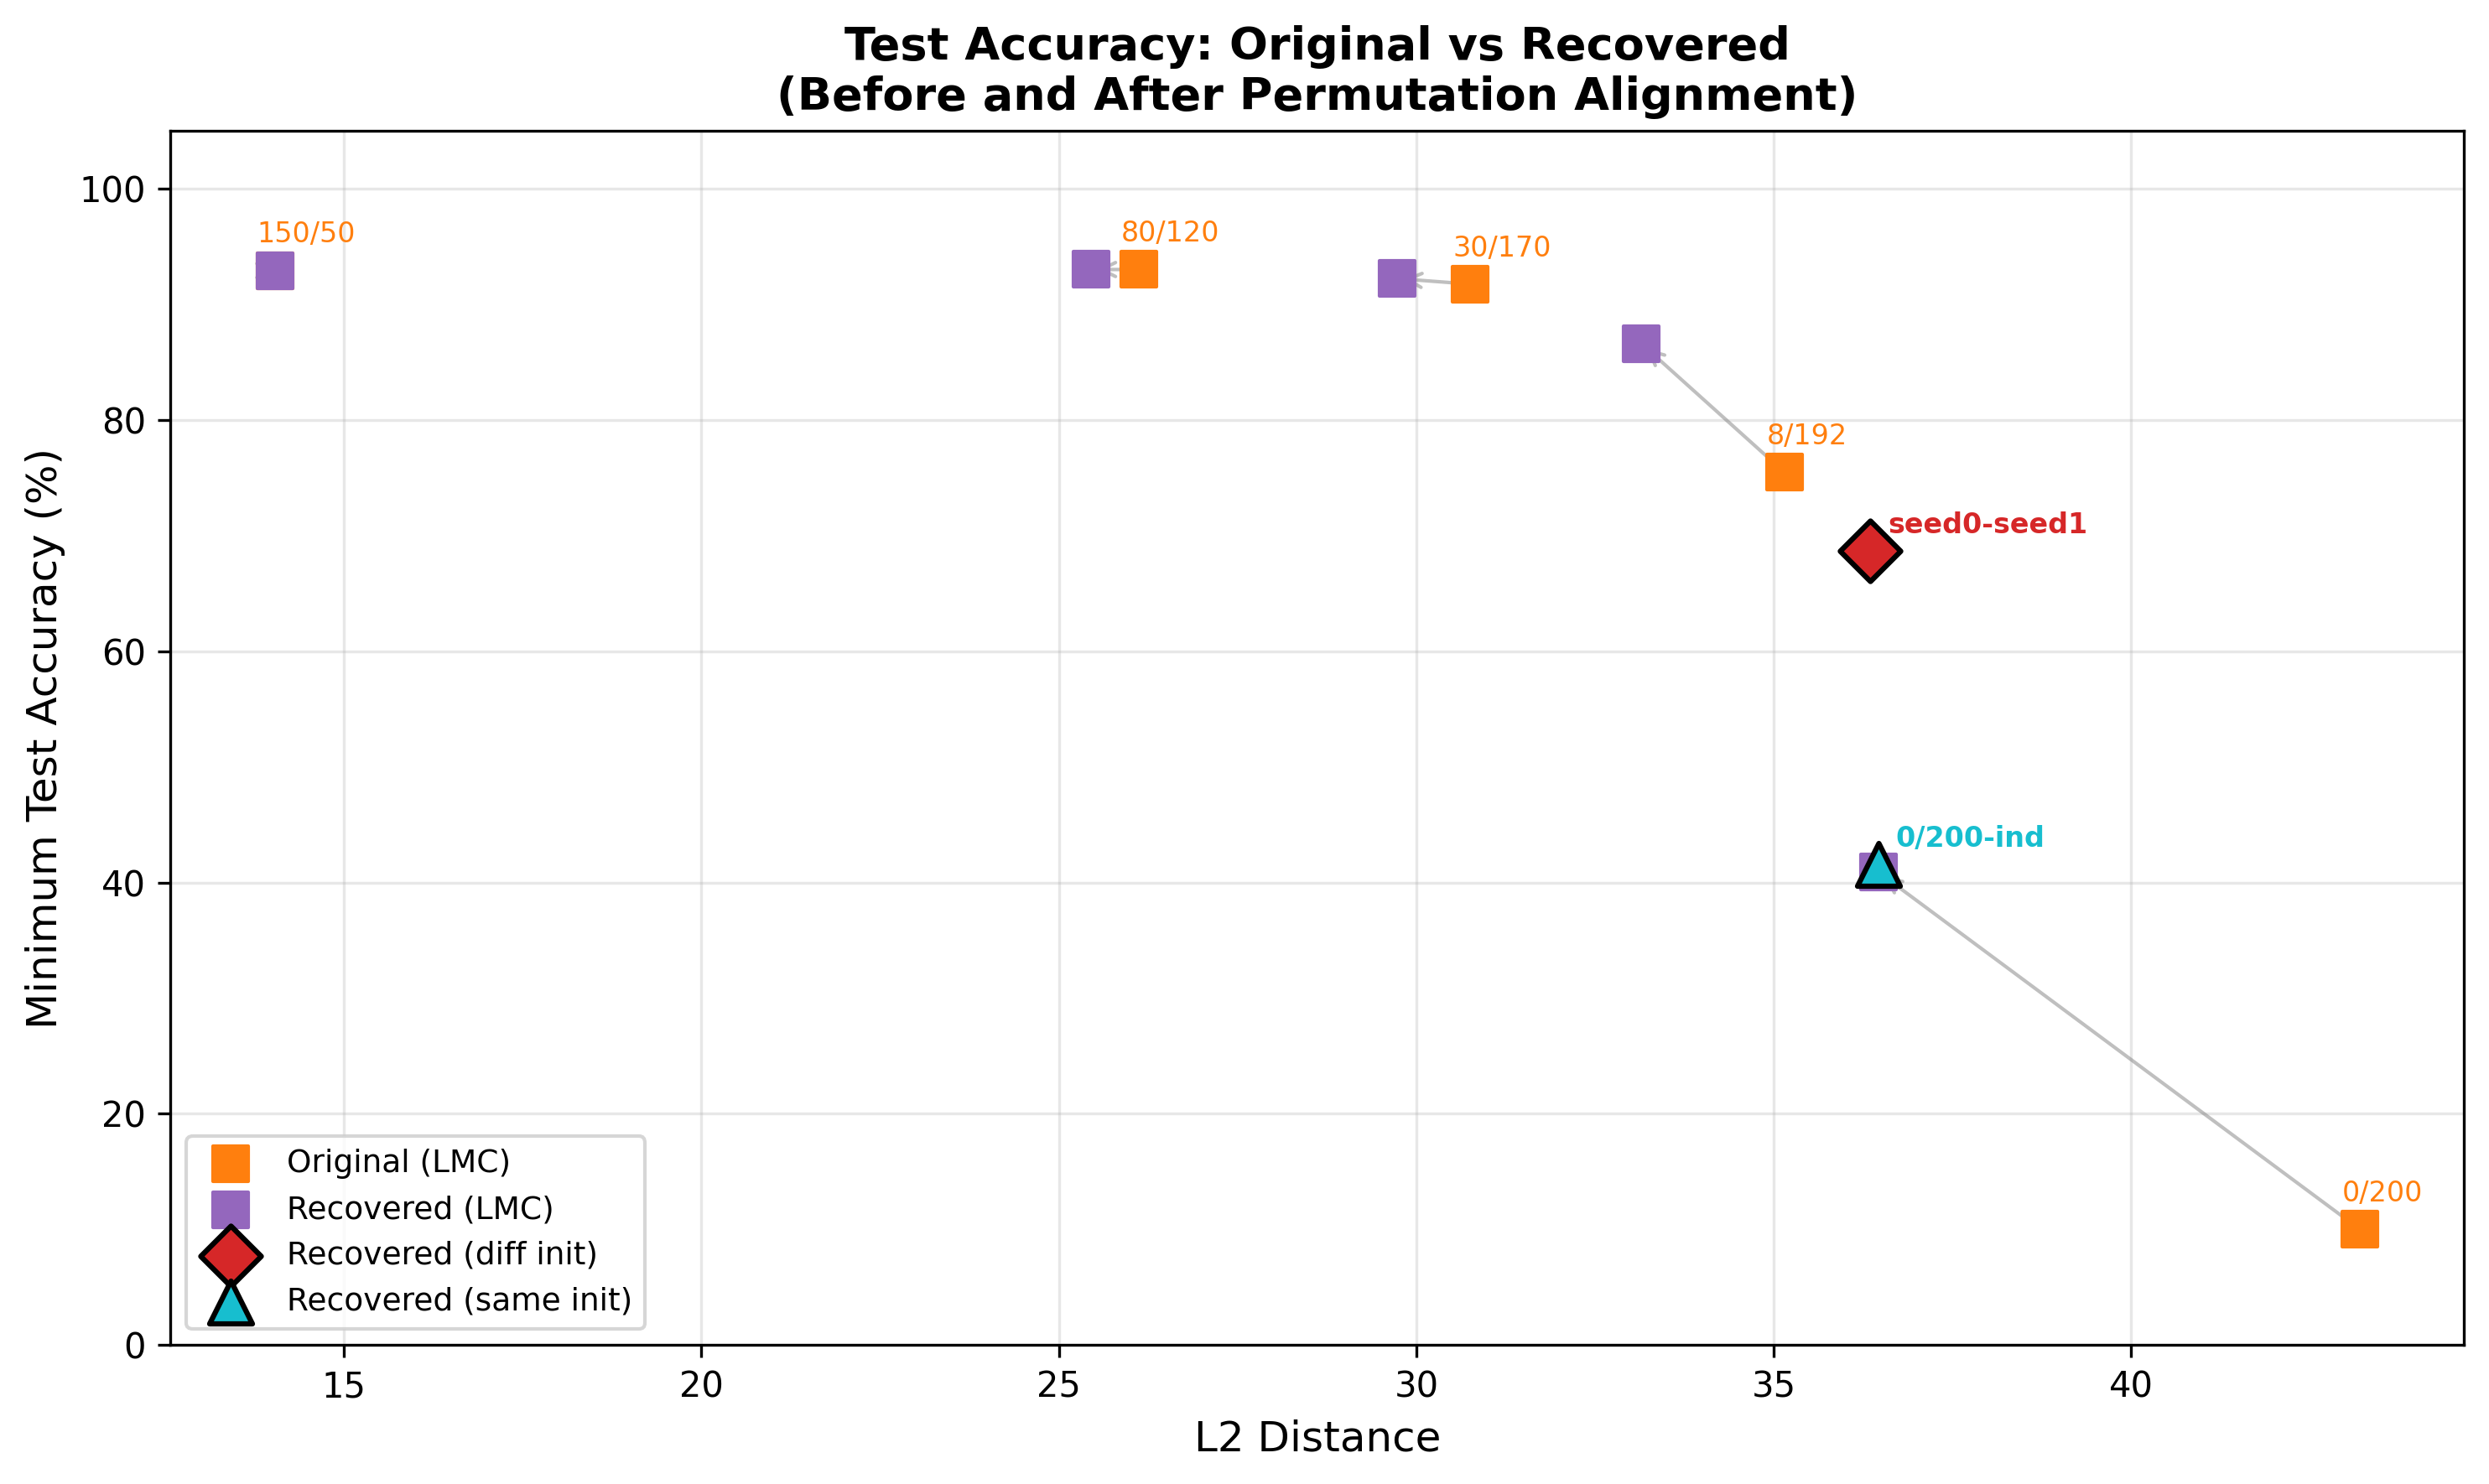
\includegraphics[width=1\linewidth]{test_accuracy.png}
    \vspace{0.5cm}
    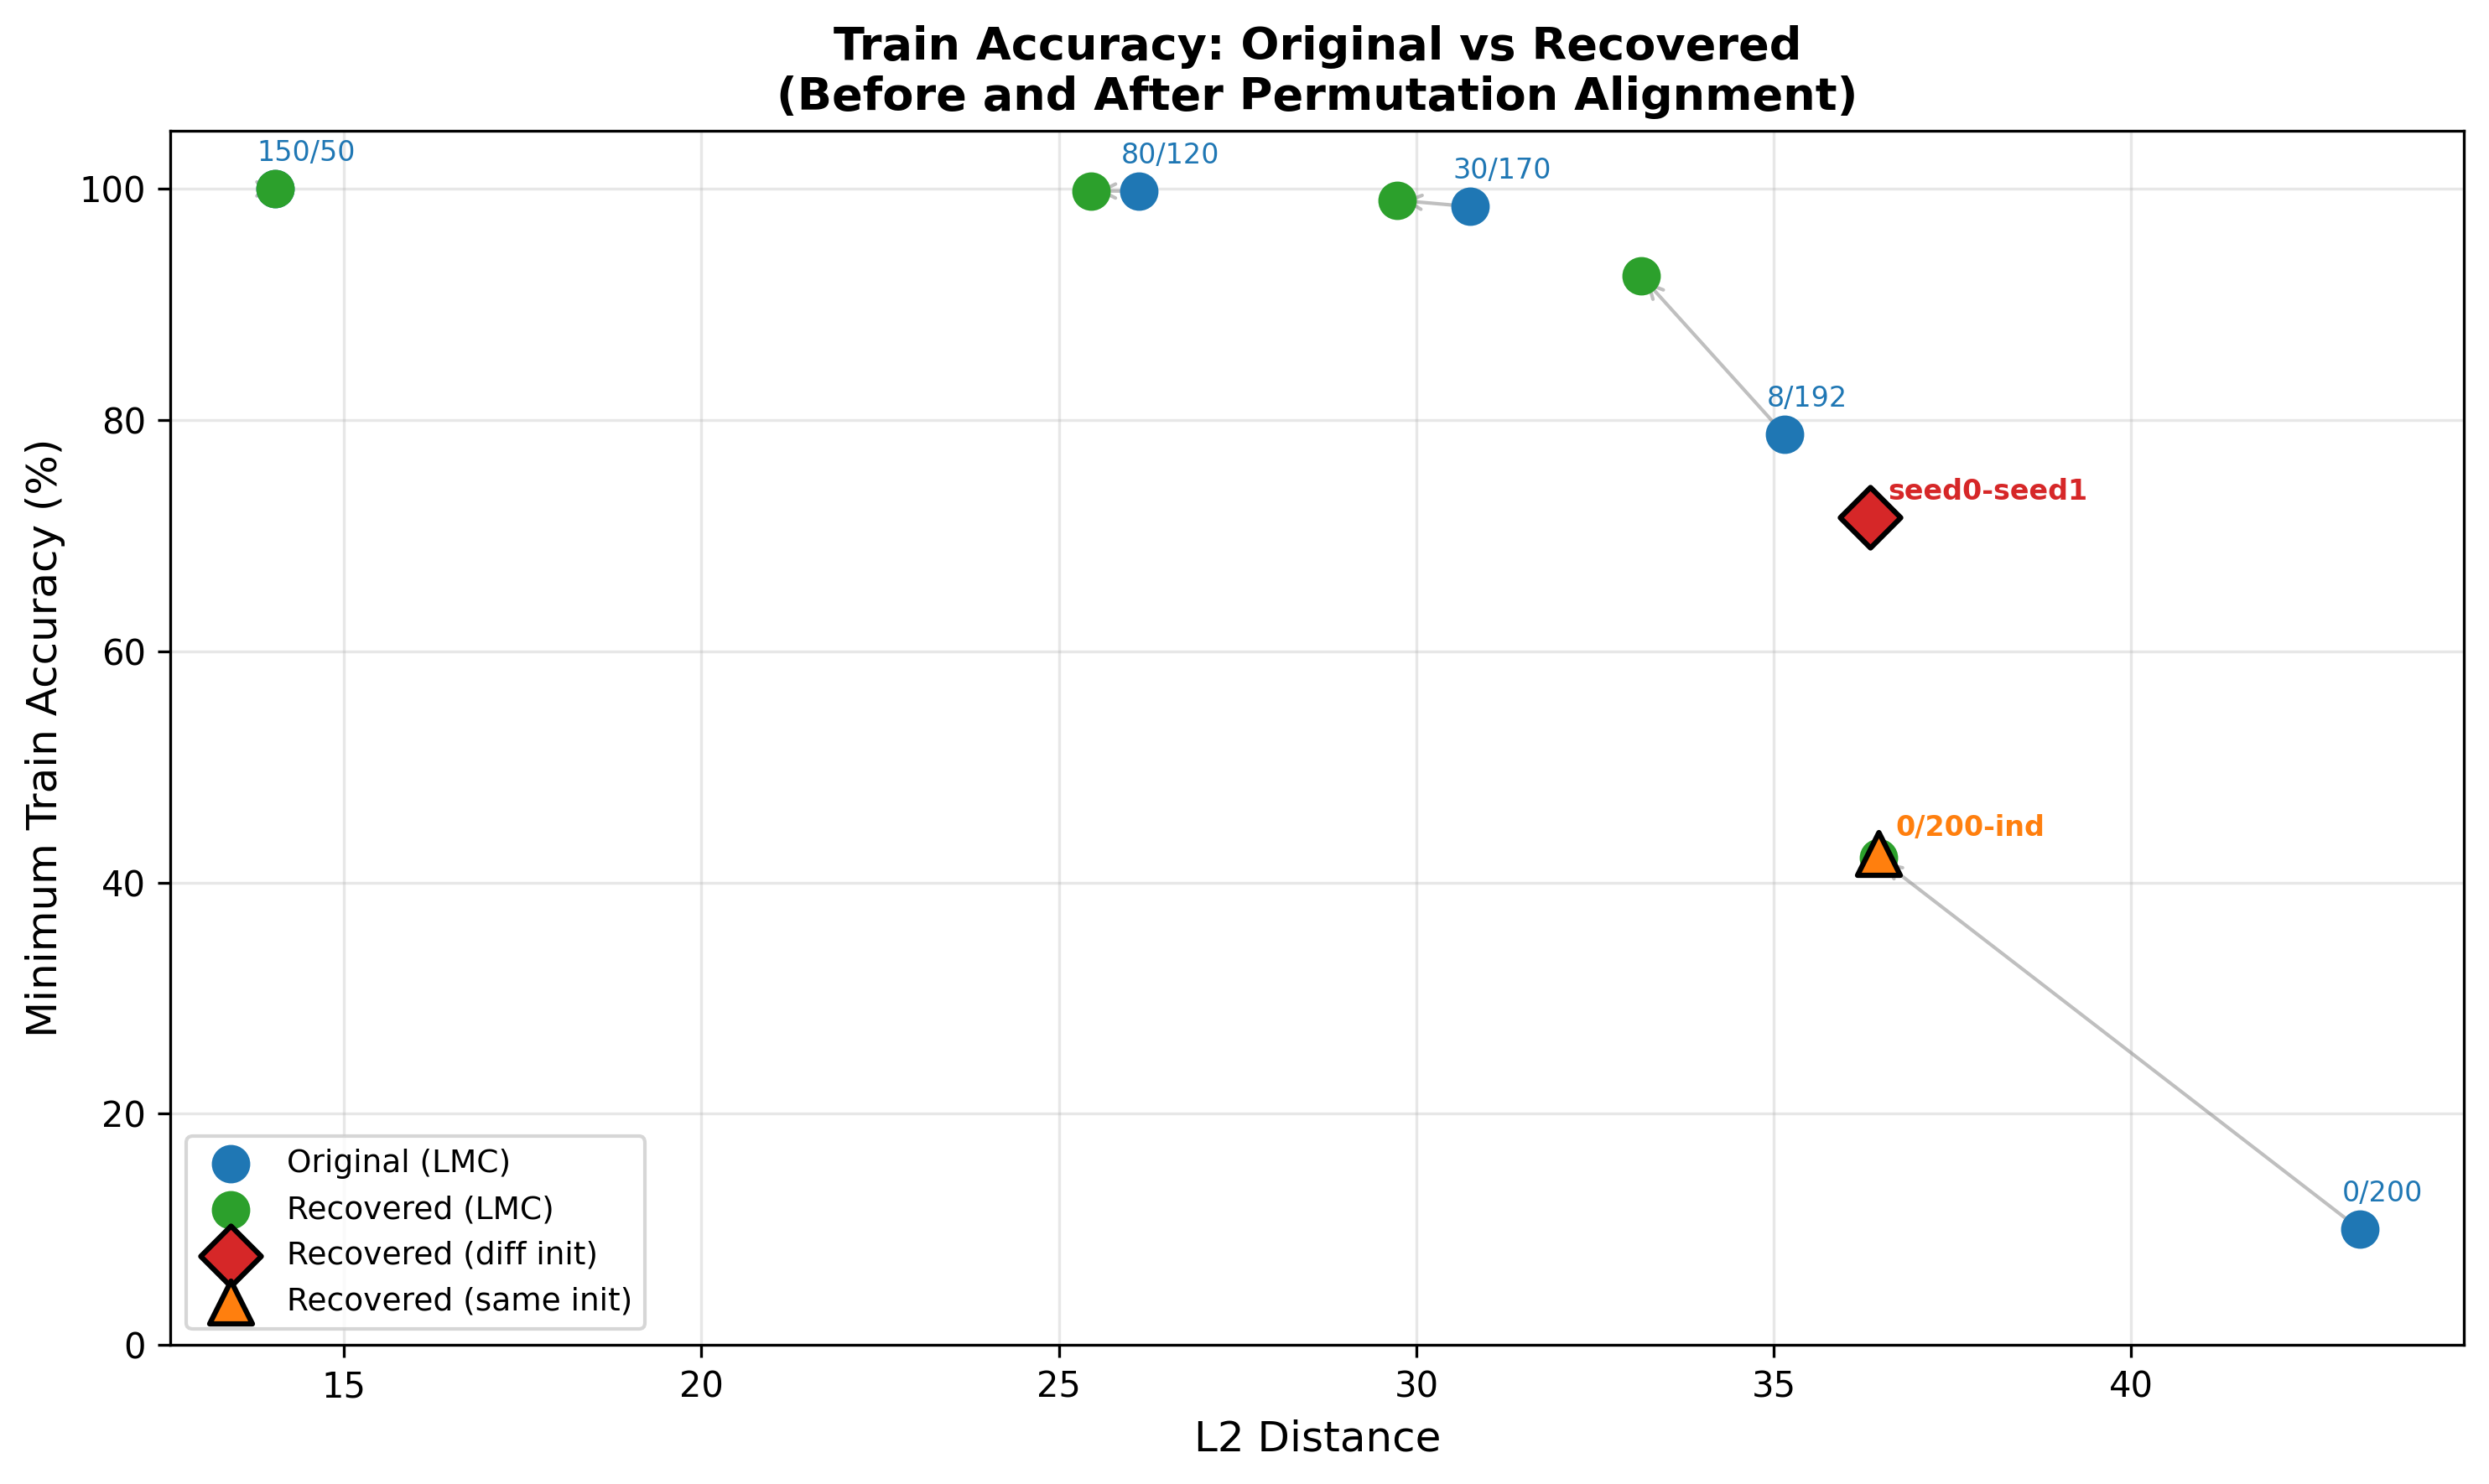
\includegraphics[width=1\linewidth]{train_accuracy.png}
    \caption{Accuracy along the linear interpolation path for the original LMC pair ($w_0 \leftrightarrow w_1$) versus the recovered pair ($w_0 \leftrightarrow w_{1,\text{rec}}$) at varying divergence levels. Top: test accuracy. Bottom: train accuracy.}
    \label{fig:accuracy-comparison}
\end{figure}


\subsection{Effect of Mode Distance on Alignment Quality}

Figure \ref{fig:accuracy-comparison} reveals a clear relationship: as the distance between $w_0$ and $w_1$ increases (corresponding to longer divergent training and weaker LMC), the alignment task becomes harder. At small distances, weight matching achieves near-perfect recovery. At larger distances approaching the independent model regime ($\sim$36), alignment quality degrades.

\begin{figure}[H]
    \centering
    
\includegraphics[width=1\linewidth]{l2 distastance recovery after permutation alignment.png}
    \caption{L2 distance recovery after permutation alignment across different divergence settings.}
    \label{fig:l2-recovery}
\end{figure}

\subsection{Key Findings}

\begin{enumerate}
    \item \textbf{Surprising over-recovery:} In every case, the recovered barrier $\text{barrier}(w_0, w_{1,\text{rec}})$ is \textit{lower} than the original $\text{barrier}(w_0, w_1)$. This suggests the alignment found a ``shortcut'' that happens to improve connectivity. The greater the barrier, the greater the improvement.
    
    \item \textbf{Independent model gap:} For independently trained models ($\text{seed}_0$, $\text{seed}_1$), the distance after alignment is $\sim$36. To create a fair comparison, we sought LMC pairs with $\|w_0 - w_1\| \approx 36$ (matching independent models). We found that at distance 35.14, the models are barely LMC-connected (barrier $\approx$ 15-20\%). \textbf{This raises the question: can we construct LMC pairs at this distance using alternative methods? If not, can we reasonably expect permutation alignment methods to bring two independently seeded models into the same LMC basin when the optimization process itself cannot even produce two modes within the same basin separated by the same distance?}

    \item \textbf{Variance Collapse Considerations:} The increased barrier at $t=0.5$ observed in our interpolations is consistent with the variance collapse phenomenon identified by Jordan et al. (2023). This same mechanism may explain our difficulty constructing LMC-connected pairs at large distances: even within the same basin (shared initialization), models that diverge significantly develop different internal activation statistics. When linearly interpolated, these mismatched statistics cause variance collapse, producing high barriers despite the models being in the same basin. This suggests that LMC is not purely a property of basin membership, but also depends on the compatibility of activation statistics along the interpolation path. Future work should incorporate REPAIR to test this hypothesis—if REPAIR recovers low barriers for distant same-basin pairs but not for independently trained models, it would provide strong evidence that independent models are genuinely in different basins rather than simply suffering from variance mismatch.

\end{enumerate}

\bibliographystyle{plain}
\begin{thebibliography}{9}

\bibitem{entezari2021}
Entezari, R., Sedghi, H., Saukh, O., \& Neyshabur, B. (2021).
The role of permutation invariance in linear mode connectivity of neural networks.
\textit{ICLR 2022}.

\bibitem{ainsworth2022}
Ainsworth, S. K., Hayase, J., \& Srinivasa, S. (2022).
Git re-basin: Merging models modulo permutation symmetries.
\textit{ICLR 2023}.

\bibitem{jordan2023}
Jordan, K., Sedghi, H., Saukh, O., Entezari, R., \& Neyshabur, B. (2023).
REPAIR: REnormalizing Permuted Activations for Interpolation Repair.
\textit{ICLR 2023}.

\bibitem{zhao2025}
Zhao, H., et al. (2025).
Understanding Mode Connectivity via Parameter Space Symmetry.
\textit{ICML 2025}.

\bibitem{findthelady}
De Sousa Trias, C., et al. (2024).
Find the Lady: Permutation and Re-synchronization of Deep Neural Networks.
\textit{AAAI 2024}.

\bibitem{crisostomi2024}
Crisostomi, D., et al. (2024).
C$^2$M$^3$: Cycle-Consistent Multi-Model Merging.
\textit{arXiv preprint}.

\end{thebibliography}

\end{document}